\documentclass[12pt,twoside,openany]{memoir}
\usepackage[T1]{fontenc}
%\usepackage{tgpagella} % text only
%\usepackage{mathpazo}  % math & text
\usepackage[T1]{fontenc}
\usepackage[hidelinks]{hyperref}
\usepackage{amsmath}
\usepackage{amsthm}
\usepackage{amssymb}
\usepackage{mathtools}
\usepackage{graphicx}
%\usepackage{newpxtext}
%\usepackage{eulerpx}
%\usepackage{eucal}
\usepackage{datetime}
    \newdateformat{specialdate}{\THEYEAR\ \monthname\ \THEDAY}
\usepackage[margin=1in]{geometry}
\usepackage{fancyhdr}
    \fancyhf{}
    \pagestyle{fancy}
    \cfoot{\scriptsize \thepage}
    \fancyhead[R]{\scriptsize \rightmark}
    \fancyhead[L]{\scriptsize \leftmark}
    \renewcommand{\headrulewidth}{0pt}
    \renewcommand{\footrulewidth}{0pt} % if you also want to remove the footer rule
\usepackage{mdframed}
\mdfsetup{font=\small}

\mdfdefinestyle{mystyle}{linecolor=black }







\usepackage{thmtools}
    \declaretheoremstyle[
        spaceabove=10pt,
        spacebelow=10pt,
        headfont=\normalfont\bfseries,
        notefont=\mdseries, notebraces={(}{)},
        bodyfont=\normalfont,
        postheadspace=0.5em
        %qed=\qedsymbol
        ]{defs}

    \declaretheoremstyle[ 
        spaceabove=10pt, % space above the theorem
        spacebelow=10pt,
        headfont=\normalfont\bfseries,
        bodyfont=\normalfont\itshape,
        postheadspace=0.5em
        ]{thmstyle}
    
    \declaretheorem[
        style=thmstyle,
        numberwithin=section
    ]{theorem}

    \declaretheorem[
        style=thmstyle,
        sibling=theorem,
    ]{proposition}

    \declaretheorem[
        style=thmstyle,
        sibling=theorem,
    ]{lemma}

    \declaretheorem[
        style=thmstyle,
        sibling=theorem,
    ]{corollary}

    \declaretheorem[
        numberwithin=section,
        style=defs,
    ]{example}

    \declaretheorem[
        numberwithin=section,
        style=defs,
    ]{definition}

    \declaretheorem[
        style=defs,
        numbered=unless unique,
    ]{problem}

    \declaretheorem[
        numbered=unless unique,
        shaded={rulecolor=black,
    rulewidth=1pt, bgcolor={rgb}{1,1,1}}
    ]{axiom}

    \declaretheorem[numberwithin=section,style=defs]{note}
    \declaretheorem[numbered=no,style=defs]{question}
    \declaretheorem[numbered=no,style=defs]{recall}
    \declaretheorem[numbered=no,style=remark]{answer}
    \declaretheorem[numbered=no,style=remark]{solution}

    \declaretheorem[numbered=no,style=defs]{remark}
\usepackage{enumitem}
\usepackage{titlesec}
    \titleformat{\chapter}[display]
    {\bfseries\LARGE\raggedright}
    {Chapter {\thechapter}}
    {1ex minus .1ex}
    {\Huge}
    \titlespacing{\chapter}
    {3pc}{*3}{40pt}[3pc]

    \titleformat{\section}[block]
    {\normalfont\bfseries\Large}
    {\S\ \thesection.}{.5em}{}[]
    \titlespacing{\section}
    {0pt}{3ex plus .1ex minus .2ex}{3ex plus .1ex minus .2ex}
\usepackage[utf8x]{inputenc}
\usepackage{tikz}
\usepackage{tikz-cd}
\usepackage{wasysym}
\usepackage{pgf}
\usepackage{mmacells}
\usepackage{listings}
\usepackage{xcolor}

\definecolor{codegreen}{rgb}{0,0.6,0}
\definecolor{codegray}{rgb}{0.5,0.5,0.5}
\definecolor{codepurple}{rgb}{0.58,0,0.82}
\definecolor{backcolour}{rgb}{0.95,0.95,0.92}

\lstdefinestyle{mystyle}{
    backgroundcolor=\color{backcolour},   
    commentstyle=\color{codegreen},
    keywordstyle=\color{magenta},
    numberstyle=\tiny\color{codegray},
    stringstyle=\color{codepurple},
    basicstyle=\ttfamily\footnotesize,
    breakatwhitespace=false,         
    breaklines=true,                 
    captionpos=b,                    
    keepspaces=true,                 
    numbers=left,                    
    numbersep=5pt,                  
    showspaces=false,                
    showstringspaces=false,
    showtabs=false,                  
    tabsize=2
}

\lstset{style=mystyle}
\usepackage{fancyvrb}
\usepackage{tcolorbox}
\setlength\parindent{0pt}

% Define replacements: "what to look for" => "how to typeset it"
\mmaDefineMathReplacement[≤]{<=}{\leq}
\mmaDefineMathReplacement[≥]{>=}{\geq}
\mmaDefineMathReplacement[≠]{!=}{\neq}
\mmaDefineMathReplacement[→]{->}{\to}[2]
\mmaDefineMathReplacement[⧴]{:>}{:\hspace{-.2em}\to}[2]
\mmaDefineMathReplacement{∉}{\notin}
\mmaDefineMathReplacement{∞}{\infty}
\mmaDefineMathReplacement{𝕕}{\mathbbm{d}}

\linespread{1}
%to make the correct symbol for Sha
%\newcommand\cyr{%
%\renewcommand\rmdefault{wncyr}%
%\renewcommand\sfdefault{wncyss}%
%\renewcommand\encodingdefault{OT2}%
%\normalfont \selectfont} \DeclareTextFontCommand{\textcyr}{\cyr}


\DeclareMathOperator{\ab}{ab}
\newcommand{\absgal}{\G_{\bbQ}}
\DeclareMathOperator{\ad}{ad}
\DeclareMathOperator{\adj}{adj}
\DeclareMathOperator{\alg}{alg}
\DeclareMathOperator{\Alt}{Alt}
\DeclareMathOperator{\Ann}{Ann}
\DeclareMathOperator{\arith}{arith}
\DeclareMathOperator{\Aut}{Aut}
\DeclareMathOperator{\Be}{B}
\DeclareMathOperator{\card}{card}
\DeclareMathOperator{\Char}{char}
\DeclareMathOperator{\csp}{csp}
\DeclareMathOperator{\codim}{codim}
\DeclareMathOperator{\coker}{coker}
\DeclareMathOperator{\coh}{H}
\DeclareMathOperator{\compl}{compl}
\DeclareMathOperator{\conj}{conj}
\DeclareMathOperator{\cont}{cont}
\DeclareMathOperator{\crys}{crys}
\DeclareMathOperator{\Crys}{Crys}
\DeclareMathOperator{\cusp}{cusp}
\DeclareMathOperator{\diag}{diag}
\DeclareMathOperator{\disc}{disc}
\DeclareMathOperator{\dR}{dR}
\DeclareMathOperator{\Eis}{Eis}
\DeclareMathOperator{\End}{End}
\DeclareMathOperator{\ev}{ev}
\DeclareMathOperator{\eval}{eval}
\DeclareMathOperator{\Eq}{Eq}
\DeclareMathOperator{\Ext}{Ext}
\DeclareMathOperator{\Fil}{Fil}
\DeclareMathOperator{\Fitt}{Fitt}
\DeclareMathOperator{\Frob}{Frob}
\DeclareMathOperator{\G}{G}
\DeclareMathOperator{\Gal}{Gal}
\DeclareMathOperator{\GL}{GL}
\DeclareMathOperator{\Gr}{Gr}
\DeclareMathOperator{\Graph}{Graph}
\DeclareMathOperator{\GSp}{GSp}
\DeclareMathOperator{\GUn}{GU}
\DeclareMathOperator{\Hom}{Hom}
\DeclareMathOperator{\id}{id}
\DeclareMathOperator{\Id}{Id}
\DeclareMathOperator{\Ik}{Ik}
\DeclareMathOperator{\IM}{Im}
\DeclareMathOperator{\Image}{im}
\DeclareMathOperator{\Ind}{Ind}
\DeclareMathOperator{\Inf}{inf}
\DeclareMathOperator{\Isom}{Isom}
\DeclareMathOperator{\J}{J}
\DeclareMathOperator{\Jac}{Jac}
\DeclareMathOperator{\lcm}{lcm}
\DeclareMathOperator{\length}{length}
\DeclareMathOperator{\Log}{Log}
\DeclareMathOperator{\M}{M}
\DeclareMathOperator{\Mat}{Mat}
\DeclareMathOperator{\N}{N}
\DeclareMathOperator{\Nm}{Nm}
\DeclareMathOperator{\NIk}{N-Ik}
\DeclareMathOperator{\NSK}{N-SK}
\DeclareMathOperator{\new}{new}
\DeclareMathOperator{\obj}{obj}
\DeclareMathOperator{\old}{old}
\DeclareMathOperator{\ord}{ord}
\DeclareMathOperator{\Or}{O}
\DeclareMathOperator{\PGL}{PGL}
\DeclareMathOperator{\PGSp}{PGSp}
\DeclareMathOperator{\rank}{rank}
\DeclareMathOperator{\Rel}{Rel}
\DeclareMathOperator{\Real}{Re}
\DeclareMathOperator{\RES}{res}
\DeclareMathOperator{\Res}{Res}
%\DeclareMathOperator{\Sha}{\textcyr{Sh}}
\DeclareMathOperator{\Sel}{Sel}
\DeclareMathOperator{\semi}{ss}
\DeclareMathOperator{\sgn}{sign}
\DeclareMathOperator{\SK}{SK}
\DeclareMathOperator{\SL}{SL}
\DeclareMathOperator{\SO}{SO}
\DeclareMathOperator{\Sp}{Sp}
\DeclareMathOperator{\Span}{span}
\DeclareMathOperator{\Spec}{Spec}
\DeclareMathOperator{\spin}{spin}
\DeclareMathOperator{\st}{st}
\DeclareMathOperator{\St}{St}
\DeclareMathOperator{\SUn}{SU}
\DeclareMathOperator{\supp}{supp}
\DeclareMathOperator{\Sup}{sup}
\DeclareMathOperator{\Sym}{Sym}
\DeclareMathOperator{\Tam}{Tam}
\DeclareMathOperator{\tors}{tors}
\DeclareMathOperator{\tr}{tr}
\DeclareMathOperator{\un}{un}
\DeclareMathOperator{\Un}{U}
\DeclareMathOperator{\val}{val}
\DeclareMathOperator{\vol}{vol}

\DeclareMathOperator{\Sets}{S \mkern1.04mu e \mkern1.04mu t \mkern1.04mu s}
    \newcommand{\cSets}{\scalebox{1.02}{\contour{black}{$\Sets$}}}
    
\DeclareMathOperator{\Groups}{G \mkern1.04mu r \mkern1.04mu o \mkern1.04mu u \mkern1.04mu p \mkern1.04mu s}
    \newcommand{\cGroups}{\scalebox{1.02}{\contour{black}{$\Groups$}}}

\DeclareMathOperator{\TTop}{T \mkern1.04mu o \mkern1.04mu p}
    \newcommand{\cTop}{\scalebox{1.02}{\contour{black}{$\TTop$}}}

\DeclareMathOperator{\Htp}{H \mkern1.04mu t \mkern1.04mu p}
    \newcommand{\cHtp}{\scalebox{1.02}{\contour{black}{$\Htp$}}}

\DeclareMathOperator{\Mod}{M \mkern1.04mu o \mkern1.04mu d}
    \newcommand{\cMod}{\scalebox{1.02}{\contour{black}{$\Mod$}}}

\DeclareMathOperator{\Ab}{A \mkern1.04mu b}
    \newcommand{\cAb}{\scalebox{1.02}{\contour{black}{$\Ab$}}}

\DeclareMathOperator{\Rings}{R \mkern1.04mu i \mkern1.04mu n \mkern1.04mu g \mkern1.04mu s}
    \newcommand{\cRings}{\scalebox{1.02}{\contour{black}{$\Rings$}}}

\DeclareMathOperator{\ComRings}{C \mkern1.04mu o \mkern1.04mu m \mkern1.04mu R \mkern1.04mu i \mkern1.04mu n \mkern1.04mu g \mkern1.04mu s}
    \newcommand{\cComRings}{\scalebox{1.05}{\contour{black}{$\ComRings$}}}

\DeclareMathOperator{\hHom}{H \mkern1.04mu o \mkern1.04mu m}
    \newcommand{\cHom}{\scalebox{1.02}{\contour{black}{$\hHom$}}}

         %  \item $\cGroups$
          %  \item $\cTop$
          %  \item $\cHtp$
          %  \item $\cMod$




\renewcommand{\k}{\kappa}
\newcommand{\Ff}{F_{f}}
\newcommand{\ts}{\,^{t}\!}


%Mathcal

\newcommand{\cA}{\mathcal{A}}
\newcommand{\cB}{\mathcal{B}}
\newcommand{\cC}{\mathcal{C}}
\newcommand{\cD}{\mathcal{D}}
\newcommand{\cE}{\mathcal{E}}
\newcommand{\cF}{\mathcal{F}}
\newcommand{\cG}{\mathcal{G}}
\newcommand{\cH}{\mathcal{H}}
\newcommand{\cI}{\mathcal{I}}
\newcommand{\cJ}{\mathcal{J}}
\newcommand{\cK}{\mathcal{K}}
\newcommand{\cL}{\mathcal{L}}
\newcommand{\cM}{\mathcal{M}}
\newcommand{\cN}{\mathcal{N}}
\newcommand{\cO}{\mathcal{O}}
\newcommand{\cP}{\mathcal{P}}
\newcommand{\cQ}{\mathcal{Q}}
\newcommand{\cR}{\mathcal{R}}
\newcommand{\cS}{\mathcal{S}}
\newcommand{\cT}{\mathcal{T}}
\newcommand{\cU}{\mathcal{U}}
\newcommand{\cV}{\mathcal{V}}
\newcommand{\cW}{\mathcal{W}}
\newcommand{\cX}{\mathcal{X}}
\newcommand{\cY}{\mathcal{Y}}
\newcommand{\cZ}{\mathcal{Z}}


%mathfrak (missing \fi)

\newcommand{\fa}{\mathfrak{a}}
\newcommand{\fA}{\mathfrak{A}}
\newcommand{\fb}{\mathfrak{b}}
\newcommand{\fB}{\mathfrak{B}}
\newcommand{\fc}{\mathfrak{c}}
\newcommand{\fC}{\mathfrak{C}}
\newcommand{\fd}{\mathfrak{d}}
\newcommand{\fD}{\mathfrak{D}}
\newcommand{\fe}{\mathfrak{e}}
\newcommand{\fE}{\mathfrak{E}}
\newcommand{\ff}{\mathfrak{f}}
\newcommand{\fF}{\mathfrak{F}}
\newcommand{\fg}{\mathfrak{g}}
\newcommand{\fG}{\mathfrak{G}}
\newcommand{\fh}{\mathfrak{h}}
\newcommand{\fH}{\mathfrak{H}}
\newcommand{\fI}{\mathfrak{I}}
\newcommand{\fj}{\mathfrak{j}}
\newcommand{\fJ}{\mathfrak{J}}
\newcommand{\fk}{\mathfrak{k}}
\newcommand{\fK}{\mathfrak{K}}
\newcommand{\fl}{\mathfrak{l}}
\newcommand{\fL}{\mathfrak{L}}
\newcommand{\fm}{\mathfrak{m}}
\newcommand{\fM}{\mathfrak{M}}
\newcommand{\fn}{\mathfrak{n}}
\newcommand{\fN}{\mathfrak{N}}
\newcommand{\fo}{\mathfrak{o}}
\newcommand{\fO}{\mathfrak{O}}
\newcommand{\fp}{\mathfrak{p}}
\newcommand{\fP}{\mathfrak{P}}
\newcommand{\fq}{\mathfrak{q}}
\newcommand{\fQ}{\mathfrak{Q}}
\newcommand{\fr}{\mathfrak{r}}
\newcommand{\fR}{\mathfrak{R}}
\newcommand{\fs}{\mathfrak{s}}
\newcommand{\fS}{\mathfrak{S}}
\newcommand{\ft}{\mathfrak{t}}
\newcommand{\fT}{\mathfrak{T}}
\newcommand{\fu}{\mathfrak{u}}
\newcommand{\fU}{\mathfrak{U}}
\newcommand{\fv}{\mathfrak{v}}
\newcommand{\fV}{\mathfrak{V}}
\newcommand{\fw}{\mathfrak{w}}
\newcommand{\fW}{\mathfrak{W}}
\newcommand{\fx}{\mathfrak{x}}
\newcommand{\fX}{\mathfrak{X}}
\newcommand{\fy}{\mathfrak{y}}
\newcommand{\fY}{\mathfrak{Y}}
\newcommand{\fz}{\mathfrak{z}}
\newcommand{\fZ}{\mathfrak{Z}}


%mathbf

\newcommand{\bfA}{\mathbf{A}}
\newcommand{\bfB}{\mathbf{B}}
\newcommand{\bfC}{\mathbf{C}}
\newcommand{\bfD}{\mathbf{D}}
\newcommand{\bfE}{\mathbf{E}}
\newcommand{\bfF}{\mathbf{F}}
\newcommand{\bfG}{\mathbf{G}}
\newcommand{\bfH}{\mathbf{H}}
\newcommand{\bfI}{\mathbf{I}}
\newcommand{\bfJ}{\mathbf{J}}
\newcommand{\bfK}{\mathbf{K}}
\newcommand{\bfL}{\mathbf{L}}
\newcommand{\bfM}{\mathbf{M}}
\newcommand{\bfN}{\mathbf{N}}
\newcommand{\bfO}{\mathbf{O}}
\newcommand{\bfP}{\mathbf{P}}
\newcommand{\bfQ}{\mathbf{Q}}
\newcommand{\bfR}{\mathbf{R}}
\newcommand{\bfS}{\mathbf{S}}
\newcommand{\bfT}{\mathbf{T}}
\newcommand{\bfU}{\mathbf{U}}
\newcommand{\bfV}{\mathbf{V}}
\newcommand{\bfW}{\mathbf{W}}
\newcommand{\bfX}{\mathbf{X}}
\newcommand{\bfY}{\mathbf{Y}}
\newcommand{\bfZ}{\mathbf{Z}}

\newcommand{\bfa}{\mathbf{a}}
\newcommand{\bfb}{\mathbf{b}}
\newcommand{\bfc}{\mathbf{c}}
\newcommand{\bfd}{\mathbf{d}}
\newcommand{\bfe}{\mathbf{e}}
\newcommand{\bff}{\mathbf{f}}
\newcommand{\bfg}{\mathbf{g}}
\newcommand{\bfh}{\mathbf{h}}
\newcommand{\bfi}{\mathbf{i}}
\newcommand{\bfj}{\mathbf{j}}
\newcommand{\bfk}{\mathbf{k}}
\newcommand{\bfl}{\mathbf{l}}
\newcommand{\bfm}{\mathbf{m}}
\newcommand{\bfn}{\mathbf{n}}
\newcommand{\bfo}{\mathbf{o}}
\newcommand{\bfp}{\mathbf{p}}
\newcommand{\bfq}{\mathbf{q}}
\newcommand{\bfr}{\mathbf{r}}
\newcommand{\bfs}{\mathbf{s}}
\newcommand{\bft}{\mathbf{t}}
\newcommand{\bfu}{\mathbf{u}}
\newcommand{\bfv}{\mathbf{v}}
\newcommand{\bfw}{\mathbf{w}}
\newcommand{\bfx}{\mathbf{x}}
\newcommand{\bfy}{\mathbf{y}}
\newcommand{\bfz}{\mathbf{z}}

%blackboard bold

\newcommand{\bbA}{\mathbb{A}}
\newcommand{\bbB}{\mathbb{B}}
\newcommand{\bbC}{\mathbb{C}}
\newcommand{\bbD}{\mathbb{D}}
\newcommand{\bbE}{\mathbb{E}}
\newcommand{\bbF}{\mathbb{F}}
\newcommand{\bbG}{\mathbb{G}}
\newcommand{\bbH}{\mathbb{H}}
\newcommand{\bbI}{\mathbb{I}}
\newcommand{\bbJ}{\mathbb{J}}
\newcommand{\bbK}{\mathbb{K}}
\newcommand{\bbL}{\mathbb{L}}
\newcommand{\bbM}{\mathbb{M}}
\newcommand{\bbN}{\mathbb{N}}
\newcommand{\bbO}{\mathbb{O}}
\newcommand{\bbP}{\mathbb{P}}
\newcommand{\bbQ}{\mathbb{Q}}
\newcommand{\bbR}{\mathbb{R}}
\newcommand{\bbS}{\mathbb{S}}
\newcommand{\bbT}{\mathbb{T}}
\newcommand{\bbU}{\mathbb{U}}
\newcommand{\bbV}{\mathbb{V}}
\newcommand{\bbW}{\mathbb{W}}
\newcommand{\bbX}{\mathbb{X}}
\newcommand{\bbY}{\mathbb{Y}}
\newcommand{\bbZ}{\mathbb{Z}}

\newcommand{\bmat}{\left( \begin{matrix}}
\newcommand{\emat}{\end{matrix} \right)}

\newcommand{\pmat}{\left( \begin{smallmatrix}}
\newcommand{\epmat}{\end{smallmatrix} \right)}

\newcommand{\lat}{\mathscr{L}}
\newcommand{\mat}[4]{\begin{pmatrix}{#1}&{#2}\\{#3}&{#4}\end{pmatrix}}
\newcommand{\ov}[1]{\overline{#1}}
\newcommand{\res}[1]{\underset{#1}{\RES}\,}
\newcommand{\up}{\upsilon}

\newcommand{\tac}{\textasteriskcentered}

%mahesh macros
\newcommand{\tm}{\textrm}

%Comments
\newcommand{\com}[1]{\vspace{5 mm}\par \noindent
\marginpar{\textsc{Comment}} \framebox{\begin{minipage}[c]{0.95
\textwidth} \tt #1 \end{minipage}}\vspace{5 mm}\par}

\newcommand{\Bmu}{\mbox{$\raisebox{-0.59ex}
  {$l$}\hspace{-0.18em}\mu\hspace{-0.88em}\raisebox{-0.98ex}{\scalebox{2}
  {$\color{white}.$}}\hspace{-0.416em}\raisebox{+0.88ex}
  {$\color{white}.$}\hspace{0.46em}$}{}}  %need graphicx and xcolor. this produces blackboard bold mu 

\newcommand{\hooktwoheadrightarrow}{%
  \hookrightarrow\mathrel{\mspace{-15mu}}\rightarrow
}

\makeatletter
\newcommand{\xhooktwoheadrightarrow}[2][]{%
  \lhook\joinrel
  \ext@arrow 0359\rightarrowfill@ {#1}{#2}%
  \mathrel{\mspace{-15mu}}\rightarrow
}
\makeatother

\renewcommand{\geq}{\geqslant}
    \renewcommand{\leq}{\leqslant}
    
    \newcommand{\bone}{\mathbf{1}}
    \newcommand{\sign}{\mathrm{sign}}
    \newcommand{\eps}{\varepsilon}
    \newcommand{\textui}[1]{\uline{\textit{#1}}}
    
    %\newcommand{\ov}{\overline}
    %\newcommand{\un}{\underline}
    \newcommand{\fin}{\mathrm{fin}}
    
    \newcommand{\chnum}{\titleformat
    {\chapter} % command
    [display] % shape
    {\centering} % format
    {\Huge \color{black} \shadowbox{\thechapter}} % label
    {-0.5em} % sep (space between the number and title)
    {\LARGE \color{black} \underline} % before-code
    }
    
    \newcommand{\chunnum}{\titleformat
    {\chapter} % command
    [display] % shape
    {} % format
    {} % label
    {0em} % sep
    { \begin{flushright} \begin{tabular}{r}  \Huge \color{black}
    } % before-code
    [
    \end{tabular} \end{flushright} \normalsize
    ] % after-code
    }

\newcommand{\littletaller}{\mathchoice{\vphantom{\big|}}{}{}{}}
\newcommand\restr[2]{{% we make the whole thing an ordinary symbol
  \left.\kern-\nulldelimiterspace % automatically resize the bar with \right
  #1 % the function
  \littletaller % pretend it's a little taller at normal size
  \right|_{#2} % this is the delimiter
  }}

\newcommand{\mtext}[1]{\hspace{6pt}\text{#1}\hspace{6pt}}

%This adds a "front cover" page.
%{\thispagestyle{empty}
%\vspace*{\fill}
%\begin{tabular}{l}
%\begin{tabular}{l}
%\includegraphics[scale=0.24]{oxy-logo.png}
%\end{tabular} \\
%\begin{tabular}{l}
%\Large \color{black} Module Theory, Linear Algebra, and Homological Algebra \\ \Large \color{black} Gianluca Crescenzo
%\end{tabular}
%\end{tabular}
%\newpage

\begin{document}
\begin{center}
{\large Math 374 \\[0.1in]Midterm 1 \\[0.1in]}
{Name:} {\underline{Gianluca Crescenzo\hspace*{2in}}}\\[0.15in]
\end{center}
\vspace{4pt}
%%%%%%%%%%%%%%%%%%%%%%%%%%%%%%%%%%%%%%%%%%%%%%%%%%%%%%%%%%%%%
\begin{enumerate}[label = \arabic*.]
    \item \textbf{Express the numbers in the forms indicated:}
        \begin{enumerate}[label = (\alph*)]
            \item $103.456_{10}$ in base 2, keeping 8 digits to the right of the binary point. Write this in base 16 as well;
            \item $A0C.9_{16}$ in base 10;
            \item Write the number $-159$ as a 16 bit signed integer.
        \end{enumerate}
\end{enumerate}


\begin{solution}
    I've written the following Mathematica code to help solve this problem:
\begin{mmaCell}[functionlocal=y]{Code}
ClearAll[ChangeBase];
ChangeBase[n_, b_, fracDigits_] := 
    Module[{i, f, ibits, fbits, q, r, s, digit},
    i = IntegerPart[n];
    f = FractionalPart[n];
    ibits = "";
    fbits = "";
    While[i > 0, 
      {q, r} = QuotientRemainder[i, b];
      ibits = ToString[r] <> ibits;
      i = q;];
    Do[s = b*f;
      digit = Floor[s];
      fbits = fbits <> ToString[digit];
       f = s - digit, {fracDigits}];
    If[ibits == "", ibits = "0"];
    ibits <> "." <> fbits];
\end{mmaCell}

    (a) Using the \texttt{ChangeBase} module, we have:
\begin{mmaCell}[functionlocal = y]{Code}
ChangeBase[103.456, 2, 8]
ChangeBase[103.456, 16, 8]
\end{mmaCell}
\begin{mmaCell}{Output}
1 1 0 0 1 1 1 . 0 1 1 1 0 1 0 0
\end{mmaCell}
\begin{mmaCell}{Output}
6 7 . 7 4 11 12 6 10 7 14
\end{mmaCell}
    
Whence $103.456_{10} = 1100111.01110100_{2} = 67.74BC6A7E_{16}$ \nl
    \newpage
    (b) We don't need to use the above code for this part. Observe that:
        \begin{equation*}
        \begin{split}
            A0C.9_{16} 
            & = 10 \cdot 16^2 + 0 \cdot 16^1 + 12 \cdot 16^0 + 9 \cdot 16^{-1} \\
            & = 2572.5625.
        \end{split}
        \end{equation*}
        \vspace{20pt}

    (c) Using the Mathematica code again gives:
\begin{mmaCell}[functionlocal = y]{Code}
ChangeBase[159, 2, 8]
\end{mmaCell}
\begin{mmaCell}{Output}
1 0 0 1 1 1 1 1 . 0 0 0 0 0 0 0 0
\end{mmaCell}

    So we have:
        \begin{equation*}
        \begin{split}
            159 = 0000000000010011111_{2}.
        \end{split}
        \end{equation*}

    Flipping each bit gives:
        \begin{equation*}
        \begin{split}
            0000000000010011111_{2} \rightarrow 1111111111101100000_{2}.
        \end{split}
        \end{equation*}

    Finally, adding 1 gives the 16 bit signed integer expression of $-159$ using the 2's complement system.
        \begin{equation*}
        \begin{split}
            -159 = 1111111111101100001_{2}.
        \end{split}
        \end{equation*}
    


\end{solution}

%%%%%%%%%%%%%%%%%%%%%%%%%%%%%%%%%%%%%%%%%%%%%%%%%%%%%%%%%%%%%
\newpage
\vspace{25pt}
\begin{enumerate}[label = \arabic*.]
    \addtocounter{enumi}{1}
    \item \textbf{Complexity of Algorithms:}
        \begin{enumerate}[label = (\alph*)]
            \item An algorithm has complexity implicity expressed as $T(n) = 2T(n-1) + 4T(n-2)$. Determine $T(n)$ explicitly.
            \item Recall the algorithm which converts a positive integer, $n$, from its decimal form to its binary form. Determine the complexity of this algorithm, $T(n)$.
            \item Recall the algorithm which reduces an $n$ by $n$ invertible matrix to Reduced Row Echelon Form. Determine the complexity of this algorithm, $T(n)$.
        \end{enumerate}
\end{enumerate}
    
    \begin{solution}
            (a) Rewriting the equation as $T(n) - 2T(n-1) - 4T(n-2) = 0$, and guessing that $T(n) = c_1 r^n$, we obtain:
                \begin{equation*}
                \begin{split}
                    & \phantom{\implies}\hspace{6.5pt} c_1r^n - 2c_1 r^{n-1} - 4c_1r^{n-2} = 0 \\
                    & \implies c_1r^{n-2}(r^2 - 2r - 4) = 0 \\
                    & \implies r^2 - 2r - 4 = 0 \\
                    & \implies r = 1 \pm \sqrt{5}.
                \end{split}
                \end{equation*}
            Thus $T(n) = c_1 (1-\sqrt{5})^n + c_2 (1 + \sqrt{5})^n$. \nl

            (b) The algorithm for converting a positive integer $n$ from decimal to binary is essentially repeated divisions by $2$. The complexity of this algorithm is then $T(n) = T (\frac{n}{2}) + k$, where $k$ is the time it takes to perform a basic operation (in the case of this algorithm, it would be division or string concatenation). We solved this exact recurrence equation in Homework 2, and found that $T(n) = k \frac{\ln(n)}{\ln(2)} + c_1$. \nl

            (c) In the first row of our $n \times n$ matrix, we need to divide each of the $n$ elements by the pivot, resulting in exactly $n$ arithmetic operations. For each remaining $n-1$ rows, you subtract by a multiple of the pivot to zero out the first column, requiring $n^2 - n$ arithmetic operations. After handling the first column, the RREF algorithm continues on the $(n-1) \times (n-1)$ sub-matrix. Thus the complexity of the RREF algorithm is $T(n) = T(n-1) + n^2$. Observe that:
                \begin{equation*}
                \begin{split}
                    T(n) & = T(n-1) + n^2 \\
                    & = T(n-2) +(n-1)^2 + n^2 \\
                    & = T(n-3) + (n-2)^2 + (n-1)^2 + n^2 \\
                    & \vdots \\
                    & = T(1) + \sum_{i = 2}^ni^2 \\
                    & = T(1) + \frac{n(n+1)(2n+1)}{6} - 1.
                \end{split}
                \end{equation*}
    \end{solution}
    
%%%%%%%%%%%%%%%%%%%%%%%%%%%%%%%%%%%%%%%%%%%%%%%%%%%%%%%%%%%%%
\newpage
\phantom{a}
\newpage
\vspace{25pt}
\begin{enumerate}[label = \arabic*.]
    \addtocounter{enumi}{2}
    \item \textbf{Convergence rate of iterative methods.} Recall the usual Newton's method, implemented by iterating:
        \begin{equation*}
        \begin{split}
            x_{n+1} = g(x_n), \h5 \text{where} \h5 g(x) = x - \frac{f(x)}{f'(x)}.
        \end{split}
        \end{equation*}
    The usual convergence for this method to a nearby root of $f(x)$ was \textbf{quadratic}. Here, we present another iterative approach and ask you to evaluate it. For concreteness, we seek the value of $\sqrt{2}$. We use the following iterative method:
        \begin{equation*}
        \begin{split}
            x_0 = 1.0, \h9 x_{n+1} = 1 + \frac{1}{1 + x_n}.
        \end{split}
        \end{equation*}

    \begin{enumerate}[label = (\alph*)]
        \item Identify $g(x)$ for which $x_{n+1} = g(x_n)$. Set $a = \sqrt{2}$, and identify $g(a)$, $g'(a)$, and $g''(a)$.
        \item Given the error of the $n^\text{th}$ iteration $e_n$, determine the value of $e_{n+1}$ in terms of $e_n$.
        \item From the questions above, state the type of convergence achieved by this method: linear, quadratic, cubic, or other. Support your answer.
        \item Compute the first 10 iterations, keeping 15 decimal digits. Compute also the error of each iterate, and the ratio $\frac{e_{n+1}}{e_n}$. Construct a table below.
        \item Explain how the results of your table support your conclusions from parts (b) and (c).
    \end{enumerate}
\end{enumerate}
    
    \begin{solution}
        (a) We have that $g(x) = 1 + \frac{1}{1+x}$. Observe that:
            \begin{equation*}
            \begin{split}
                g(\sqrt{2}) = 1 + \frac{1}{1 + \sqrt{2}} \\
                g'(\sqrt{2}) = -\frac{1}{(1+\sqrt{2})^2} \\
                g''(\sqrt{2}) = \frac{2}{(1+\sqrt{2})^3}.
            \end{split}
            \end{equation*}

        (b) We should first verify that $\sqrt{2}$ is a fixed point:
            \begin{equation*}
            \begin{split}
                g (\sqrt{2})
                & = 1 + \frac{1}{1 + \sqrt{2}} \\
                & = 1 + \frac{1}{1 + \sqrt{2}} \cdot \frac{1 - \sqrt{2}}{1-\sqrt{2}} \\
                & = 1 + \frac{1- \sqrt{2}}{-1} \\
                & = \sqrt{2}. \\
            \end{split}
            \end{equation*}
        Now let $e_n = x_n - \sqrt{2}$. Then:
            \begin{equation*}
            \begin{split}
                e_{n+1} 
                & = x_{n+1} - \sqrt{2} \\
                & = 1 + \frac{1}{1+x_n} - \sqrt{2} \\
                & = 1 + \frac{1}{1 + x_n} - 1 - \frac{1}{1 + \sqrt{2}} \\
                & = \frac{1}{1 + x_n} - \frac{1}{ 1 + \sqrt{2}} \\
                & = \frac{\sqrt{2} - x_n}{(1+x_n)(1 + \sqrt{2})} \\
                & = \frac{-e_n}{(1+e_n + \sqrt{2})(1 + \sqrt{2})}
            \end{split}
            \end{equation*}

        (c) Consider:
            \begin{equation*}
            \begin{split}
                \frac{e_{n+1}}{e_n}
                & = \frac{x_{n+1} - \sqrt{2}}{x_n - \sqrt{2}} \\
                & = \frac{g(x_n) - g(\sqrt{2})}{x_n - \sqrt{2}} \\
                & = \ds \frac{\ds \left( \sum_{k = 0}^\infty \ds \frac{g^{(k)}(\sqrt{2})}{k!} (x_n - \sqrt{2})^k \right) - g(\sqrt{2})}{x_n - \sqrt{2}} \\
                & = \sum_{k = 1}^\infty \frac{g^{(k)}(\sqrt{2})}{k!}(x_n - \sqrt{2})^{k-1} \\
                & = \sum_{k = 1}^\infty \frac{g^{(k)}(\sqrt{2})}{k!}e_n^{k-1}.
            \end{split}
            \end{equation*}
        Multiplying $e_n$ on both sides gives:
            \begin{equation*}
            \begin{split}
                e_{n+1} = \sum_{k = 1}^\infty \frac{g^{(k)}(\sqrt{2})}{k!}e_n^k 
            \end{split}
            \end{equation*}
        Thus the convergence of this iterative method is linear. \nl

        \newpage
        (d) The following Mathematica code computes the first 10 iterations and constructs a table:

\begin{mmaCell}[functionlocal = y]{Code}
Clear["Global`*"]
it = 10;

vals = Table[0, {it + 1}];
err = Table[0, {it + 1}];

vals[[1]] = 1;
For[n = 1, n <= it, n++, 
  vals[[n + 1]] = N[1 + 1/(1 + vals[[n]]), 1000];];
For[n = 1, n <= it + 1, n++, err[[n]] = N[vals[[n]] - Sqrt[2], 1000];];

table = Table[{
    n - 1,
    NumberForm[vals[[n]], {Infinity, 15}, 
     ExponentFunction -> (Null &), NumberPadding -> {"", "0"}],
    NumberForm[err[[n]], {Infinity, 15}, ExponentFunction -> (Null &),
      NumberPadding -> {"", "0"}],
    If[n == 1, "", 
     NumberForm[err[[n]]/err[[n - 1]], {Infinity, 15}, 
      ExponentFunction -> (Null &), NumberPadding -> {"", "0"}]]
    }, {n, it + 1}];
TableForm[Prepend[table, {"n", "f[n]", "err[n]", "err[n]/err[n-1]"}]]
\end{mmaCell}
\vspace{10pt}
\begin{mmaCell}{Output}
n	    f[n]	               err[n]	                err[n]/err[n-1]
0	    1.000000000000000	   -0.414213562373095	
1	    1.500000000000000	    0.085786437626905	    -0.207106781186548
2	    1.400000000000000	   -0.014213562373095	    -0.165685424949238
3	    1.416666666666667	    0.002453104293572	    -0.172588984322123
4	    1.413793103448276	   -0.000420458924819	    -0.171398715464729
5	    1.414285714285714	    0.000072151912619	    -0.171602761554568
6	    1.414201183431953	   -0.000012378941143	    -0.171567747728501
7	    1.414215686274510	    0.000002123901415	    -0.171573755002581
8	    1.414213197969543	   -0.000000364403552	    -0.171572724312917
9	    1.414213624894870	    0.000000062521774	    -0.171572901151177
10	  1.414213551646055	   -0.000000010727040	    -0.171572870810524
\end{mmaCell}

    (e) We can see from the table that the error is increasing approximately linearly. Had it been quadratic, there would be a lot more trailing zeros. This supports our answer from part (c).

    \end{solution}
    
%%%%%%%%%%%%%%%%%%%%%%%%%%%%%%%%%%%%%%%%%%%%%%%%%%%%%%%%%%%%%
\newpage
\phantom{a}
\newpage
\vspace{25pt}
\begin{enumerate}[label = \arabic*.]
    \addtocounter{enumi}{3}
    \item \textbf{Competing Species:} A famous system of equations represents two (or more) species
    competing for resources in a given environment. Consider, for instance, skunks and
    rabbits on an island competing for food, and shelter. Let $s(t)$ and $r(t)$ represent the
    population (in tens of thousands) of skunks and rabbits at time $t$. The competing
    species equations here are:
        \begin{equation*}
        \begin{split}
            s'(t) &= 6s^2 + 4rs - 20s, \\
            r'(t) &= 30r^2 + 10rs - 125r.
        \end{split}
        \end{equation*}
    For such systems, we seek "equilibrium points". That is, values of populations of both species at which $s'(t) = r'(t) = 0$. Such points represent populations which, once achieved, remain constant. For this model, there are four such points $(r,s)$. Use Newton's method for systems of equations to determine the one such equilibrium point for which $r \neq 0$ and $ s \neq 0$.
\end{enumerate}
    
    \begin{solution}
        Given the above equations, the following Mathematica code computes the first 10 iterations of Newton's method.

\begin{mmaCell}[functionlocal = y]{Code}
Clear["Global`*"]
f1 [s_, r_] = 6 s^2 + 4 r*s - 20 s;
f2 [s_, r_] = 30 r^2 + 10 r*s - 125 r;
F[s_, r_] = {{f1[s, r]}, {f2[s, r]}};
J[s_, r_] = {{D[f1[s, r], s], D[f1[s, r], r]}, {D[f2[s, r], s], 
    D[f2[s, r], r]}};

it = 6;
sVals = Table[0, {it + 1}];
rVals = Table[0, {it + 1}];

sVals[[1]] = 1;
rVals[[1]] = 4;

For[n = 1, n <= it, n++,
  delta = 
   Inverse[J[sVals[[n]], rVals[[n]]]] . F[sVals[[n]], rVals[[n]]];
  sVals[[n + 1]] = sVals[[n]] - delta[[1, 1]];
  rVals[[n + 1]] = rVals[[n]] - delta[[2, 1]];
  ];
sol = N[Transpose[{sVals, rVals}]];

table = Table[{
    n - 1,
    NumberForm[sol[[n]], {Infinity, 15}, ExponentFunction -> (Null &),
      NumberPadding -> {"", "0"}]}, {n, 1, Length[sol]}];

TableForm[Prepend[table, {"n", "(s,r)"}]]
\end{mmaCell}
\newpage
\begin{mmaCell}{Output}
n	    (s,r)
0	    \{3.000000000000000,  4.000000000000000\}
1	    \{1.824519230769231,  3.634615384615385\}
2	    \{1.150892266024041,  3.779991223344874\}
3	    \{0.833788952159754,  3.888824678561128\}
4	    \{0.729275280895912,  3.923574123039542\}
5	    \{0.714587591547749,  3.928470803795023\}
6	    \{0.714285841760175,  3.928571386079917\}
7	    \{0.714285714285737,  3.928571428571421\}
8	    \{0.714285714285714,  3.928571428571429\}
9	    \{0.714285714285714,  3.928571428571428\}
10	  \{0.714285714285714,  3.928571428571429\}
\end{mmaCell}
    \end{solution}
    
%%%%%%%%%%%%%%%%%%%%%%%%%%%%%%%%%%%%%%%%%%%%%%%%%%%%%%%%%%%%%
\newpage
\vspace{25pt}
\begin{enumerate}[label = \arabic*.]
    \addtocounter{enumi}{4}
    \item \textbf{Eigenvalues and Eigenvectors.}
    \begin{enumerate}[label = (\alph*)]
        \item Let $A$ have eigenvalues $\lambda_1,\lambda_2,...,\lambda_n$, and corresponding eigenvectors $v_1,v_2,...,v_n$. What are the eigenvalues and eigenvectors of the matrix $2A^3 - 5A + 2I$.
        \item Consider the matrix:
        \begin{equation*}
        \begin{split}
            A = \bmat 1 & 2 & 1 \\ -2 & 9 & 3 \\ 0 & 4 & -6 \emat.
        \end{split}
        \end{equation*}
        Using only the Power Method algorithm, determine all three eigenvalues and eigenvectors.
    \end{enumerate}
\end{enumerate}
    
    \begin{solution}
        (a) Since $Av_i = \lambda_i v_i$, consider:
            \begin{equation*}
            \begin{split}
                (2A^3 - 5A + 2I)v_i 
                & = 2A^3 v_i - 5Av_i + 2Iv_i \\
                & = 2 \lambda_i^3 v_i - 5 \lambda_i v_i + 2v_i \\
                & = (2\lambda_i^3 - 5 \lambda_i + 2)v_i.
            \end{split}
            \end{equation*}
        Thus for each $i = 1,...,n$, we have that $v_i$ is an eigenvector of $2A^3 - 5A + 2I$ corresponding to the eigenvalue $2\lambda_i^3 - 5 \lambda_i + 2$.\nl
            \newpage
        (b) I wrote the following Mathematica code to help solve this problem:

\begin{mmaCell}[functionlocal = y]{Code}
Clear["Global`*"];
PowerMethod[Mat_, ic_, k_, r_, it_ : 30] := 
  Module[{A, eVects, eVals, n, table, plot},
   (*Power Method*)
   A = Mat^k + r*IdentityMatrix[3];
   eVects = Table[0, {it + 1}];
   eVals = Table[0, {it + 1}];
   eVects[[1]] = ic;
   For[n = 1, n <= it, n++, 
    eVects[[n + 1]] = (A.eVects[[n]])/N[Norm[A.eVects[[n]]], 1000];];
   For[n = 1, n <= it + 1, n++, 
    eVals[[n]] = (eVects[[n]].(A.eVects[[n]]))/(eVects[[n]].eVects[[n]]);];
   table = Table[{
      n - 1,
      NumberForm[eVects[[n]], {Infinity, 15}, 
       ExponentFunction -> (Null &), NumberPadding -> {"", "0"}], 
      NumberForm[eVals[[n]], {Infinity, 15}, 
       ExponentFunction -> (Null &), NumberPadding -> {"", "0"}], 
      NumberForm[Surd[eVals[[n]] - r, k], {Infinity, 15}, 
       ExponentFunction -> (Null &), NumberPadding -> {"", "0"}]}, {n,
       1, it + 1}];
   
   (*Gershgorin Disks*)
   (*See https://resources.wolframcloud.com/FunctionRepository/
   resources/GershgorinDisks/ *)
   plot = 
    Show[ResourceFunction["GershgorinDisks"][Mat], 
     Graphics[{Green, PointSize[0.015], 
       Point[{Surd[eVals[[it + 1]] - r, k], 0}]}], Frame -> True, 
     ImageSize -> 500];
   Column[{TableForm[
      Prepend[table, {"n", "v[n]", "E[n]", "AdjustedE[n]"}]], plot}, 
    Spacings -> 2]
   ];
\end{mmaCell}

        Since the off-diagonals of our matrix have small norm, the Gershgorin Circle Theorem says that our eigenvalues will be approximately the diagonal:
            \begin{equation*}
            \begin{split}
                \lambda_1 &\approx 1, \\
                \lambda_2 &\approx 9, \\
                \lambda_3 &\approx -6.
            \end{split}
            \end{equation*}
        Since the Power Method converges to the dominant eigenvalue of $A$, running \newline \texttt{PowerMethod[A,\{0,1,0\},1,0]} will converge to $\lambda_2$. By part (a), we saw that (non)-linear combinations of our matrix correspond to (non)-linear combinations of our eigenvalues. Considering the following shift:
            \begin{equation*}
            \begin{split}
                \lambda_1-2 &\approx -1, \\
                \lambda_2-2 &\approx 7, \\
                \lambda_3-2 &\approx -8,
            \end{split}
            \end{equation*}
        we can see that \texttt{PowerMethod[A,\{0,1,0\},1,-2]} will converge to $\lambda_3$. In order to achieve convergence to $\lambda_1$, we must consider even powers of our matrix, as \texttt{PowerMethod[A,\{0,1,0\},1,r]} for any $r \in \bfR$ will result in convergence to either $\lambda_2$ or $\lambda_3$. By considering:
            \begin{equation*}
            \begin{split}
                \lambda_1^2-50 &\approx -50, \\
                \lambda_2^2-50 &\approx 31, \\
                \lambda_3^2-50 &\approx -14,
            \end{split}
            \end{equation*}
        we have that $\lambda_1$ is now the dominant eigenvalue, whence \texttt{PowerMethod[A,\{0,1,0\},2,-50]} will converge to our final eigenvalue. Using such guesses, we can now obtain all of the eigenvalues and eigenvectors of $A$.
\begin{mmaCell}[functionlocal = y]{Code}
Mat = {{1, 2, 1}, {-2, 9, 3}, {0, 4, -6}};
PowerMethod[Mat, {0, 1, 0}, 2, -50, 30]
PowerMethod[Mat, {0, 1, 0}, 1, 0, 30]
PowerMethod[Mat, {0, 1, 0}, 1, -2, 30]
\end{mmaCell}

\begin{mmaCell}{Output}

\end{mmaCell}
\h9\h9\h9\h9\h9\h9\h9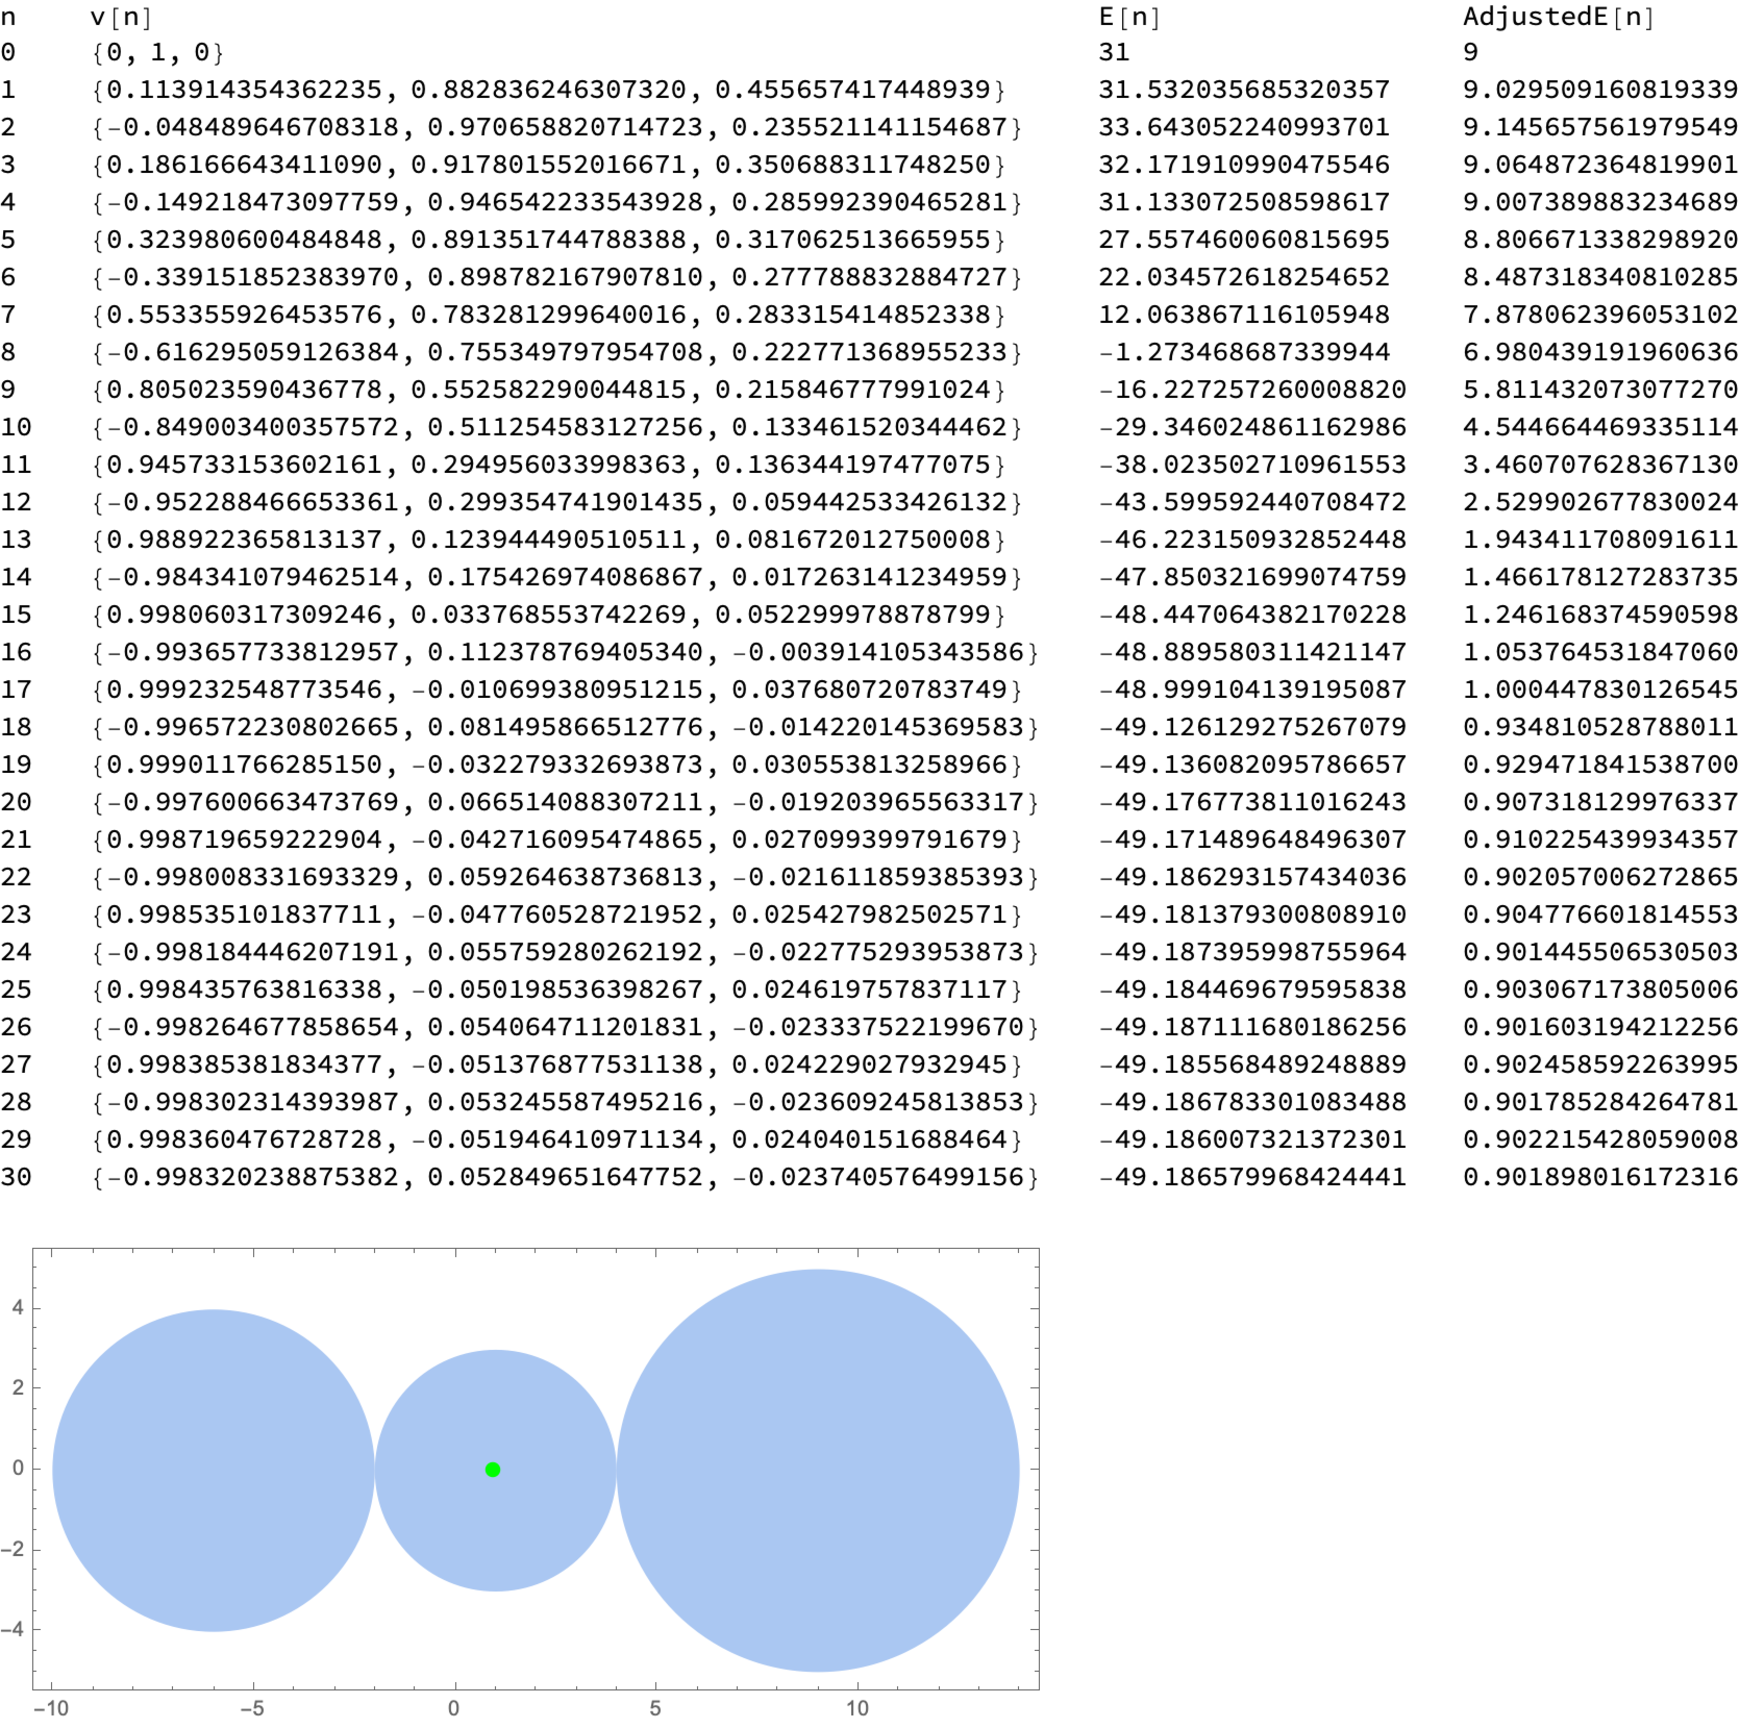
\includegraphics[scale=0.5]{hw50}

\newpage
\begin{mmaCell}{Output}

\end{mmaCell}
\h9\h9\h9\h9\h9\h9\h9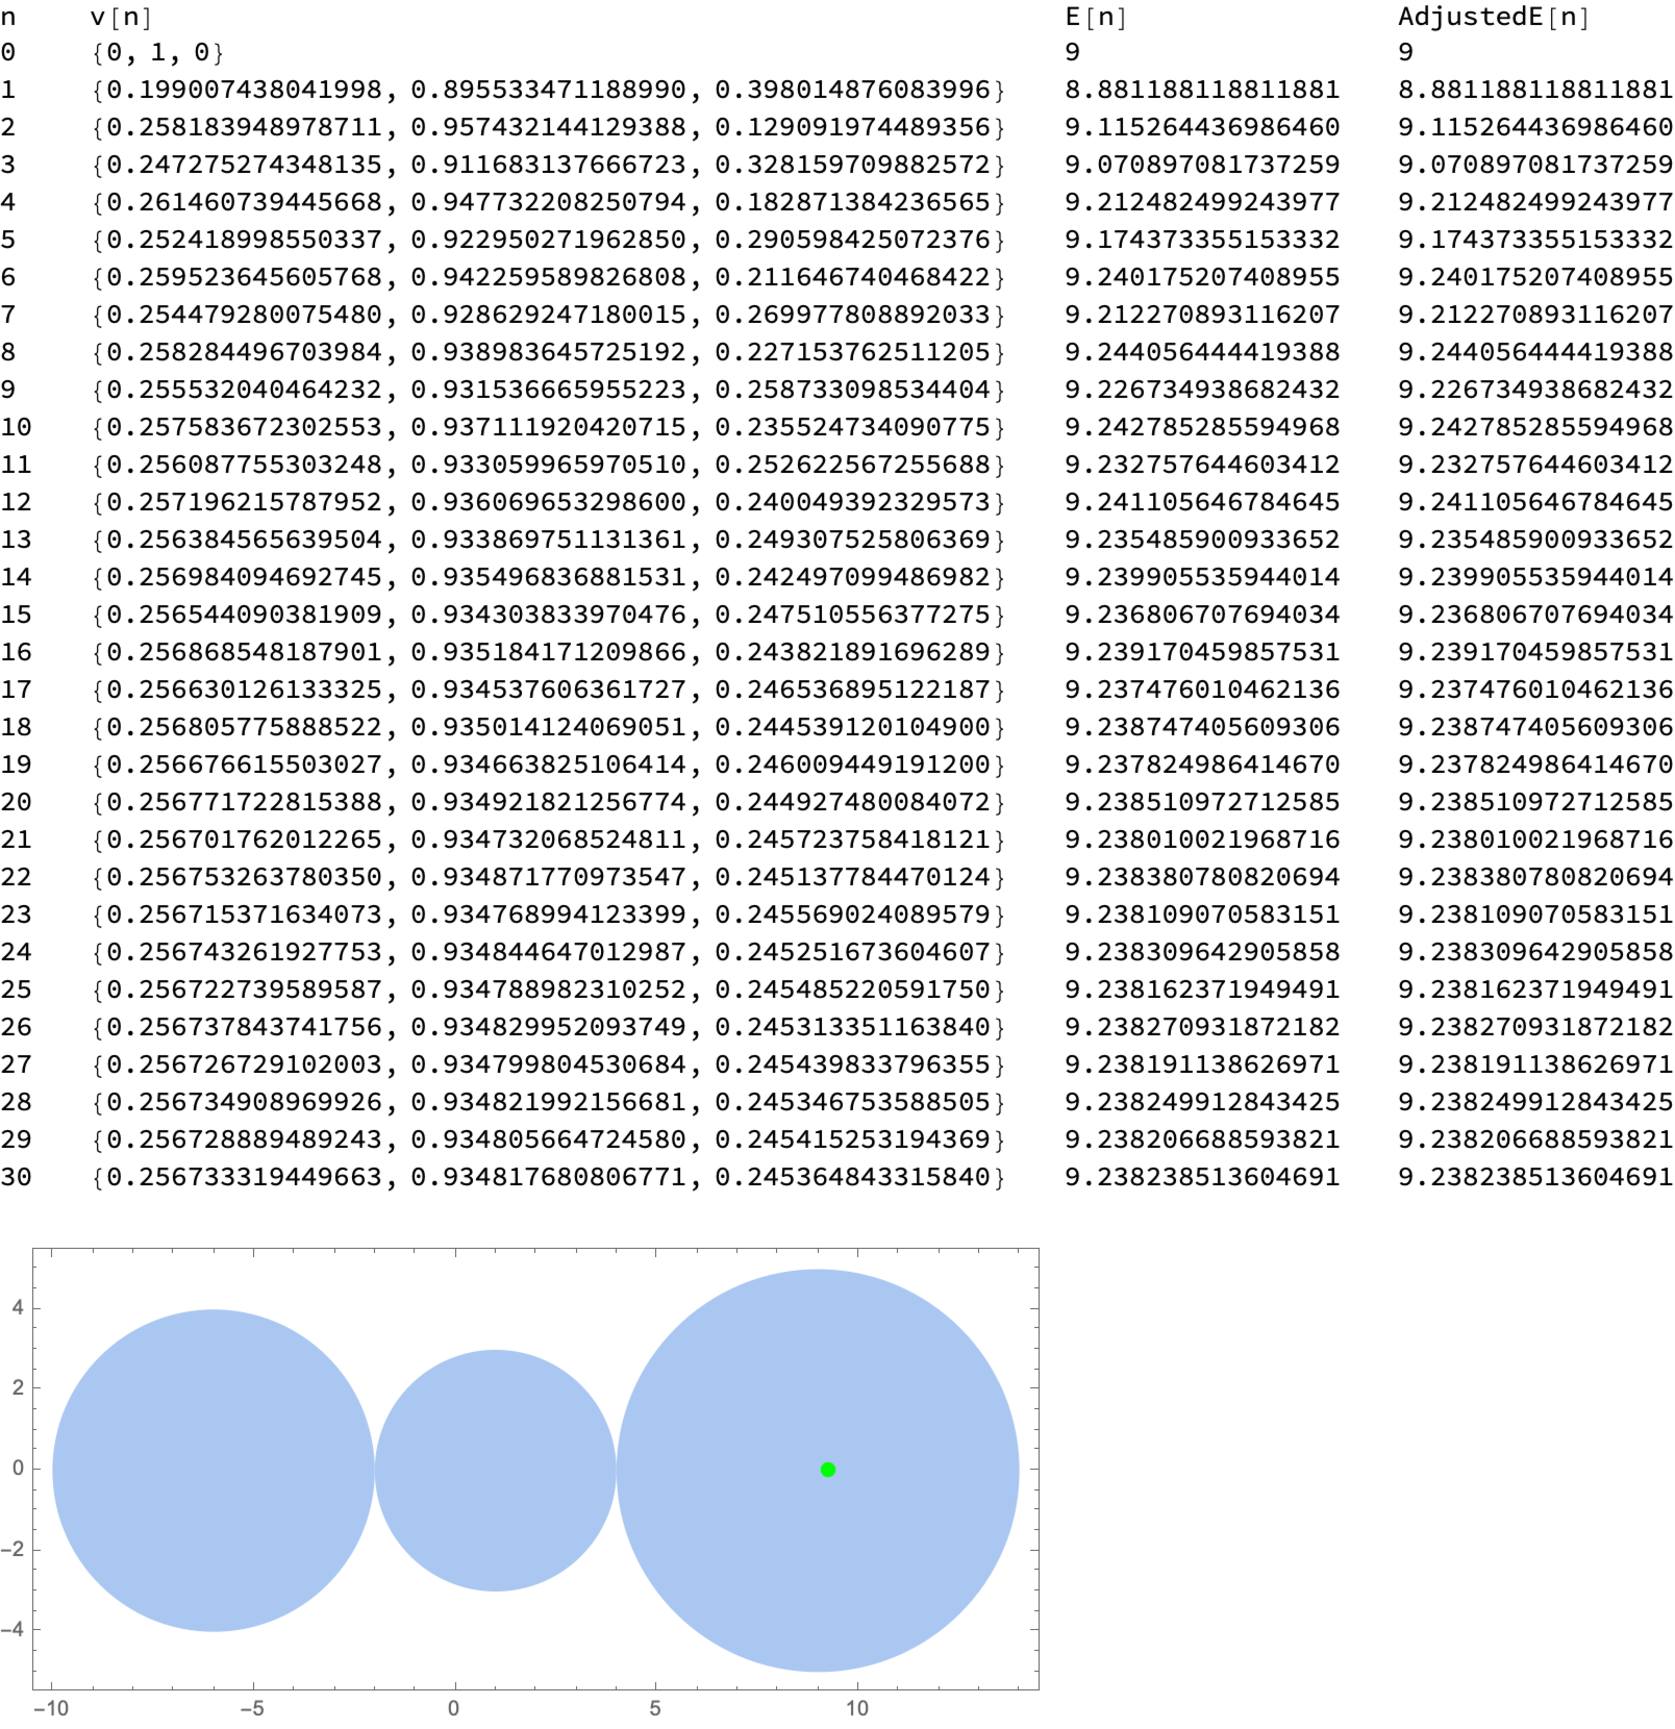
\includegraphics[scale=0.5]{problem51}

\newpage
\begin{mmaCell}{Output}
 
\end{mmaCell}
\h9\h9\h9\h9\h9\h9\h9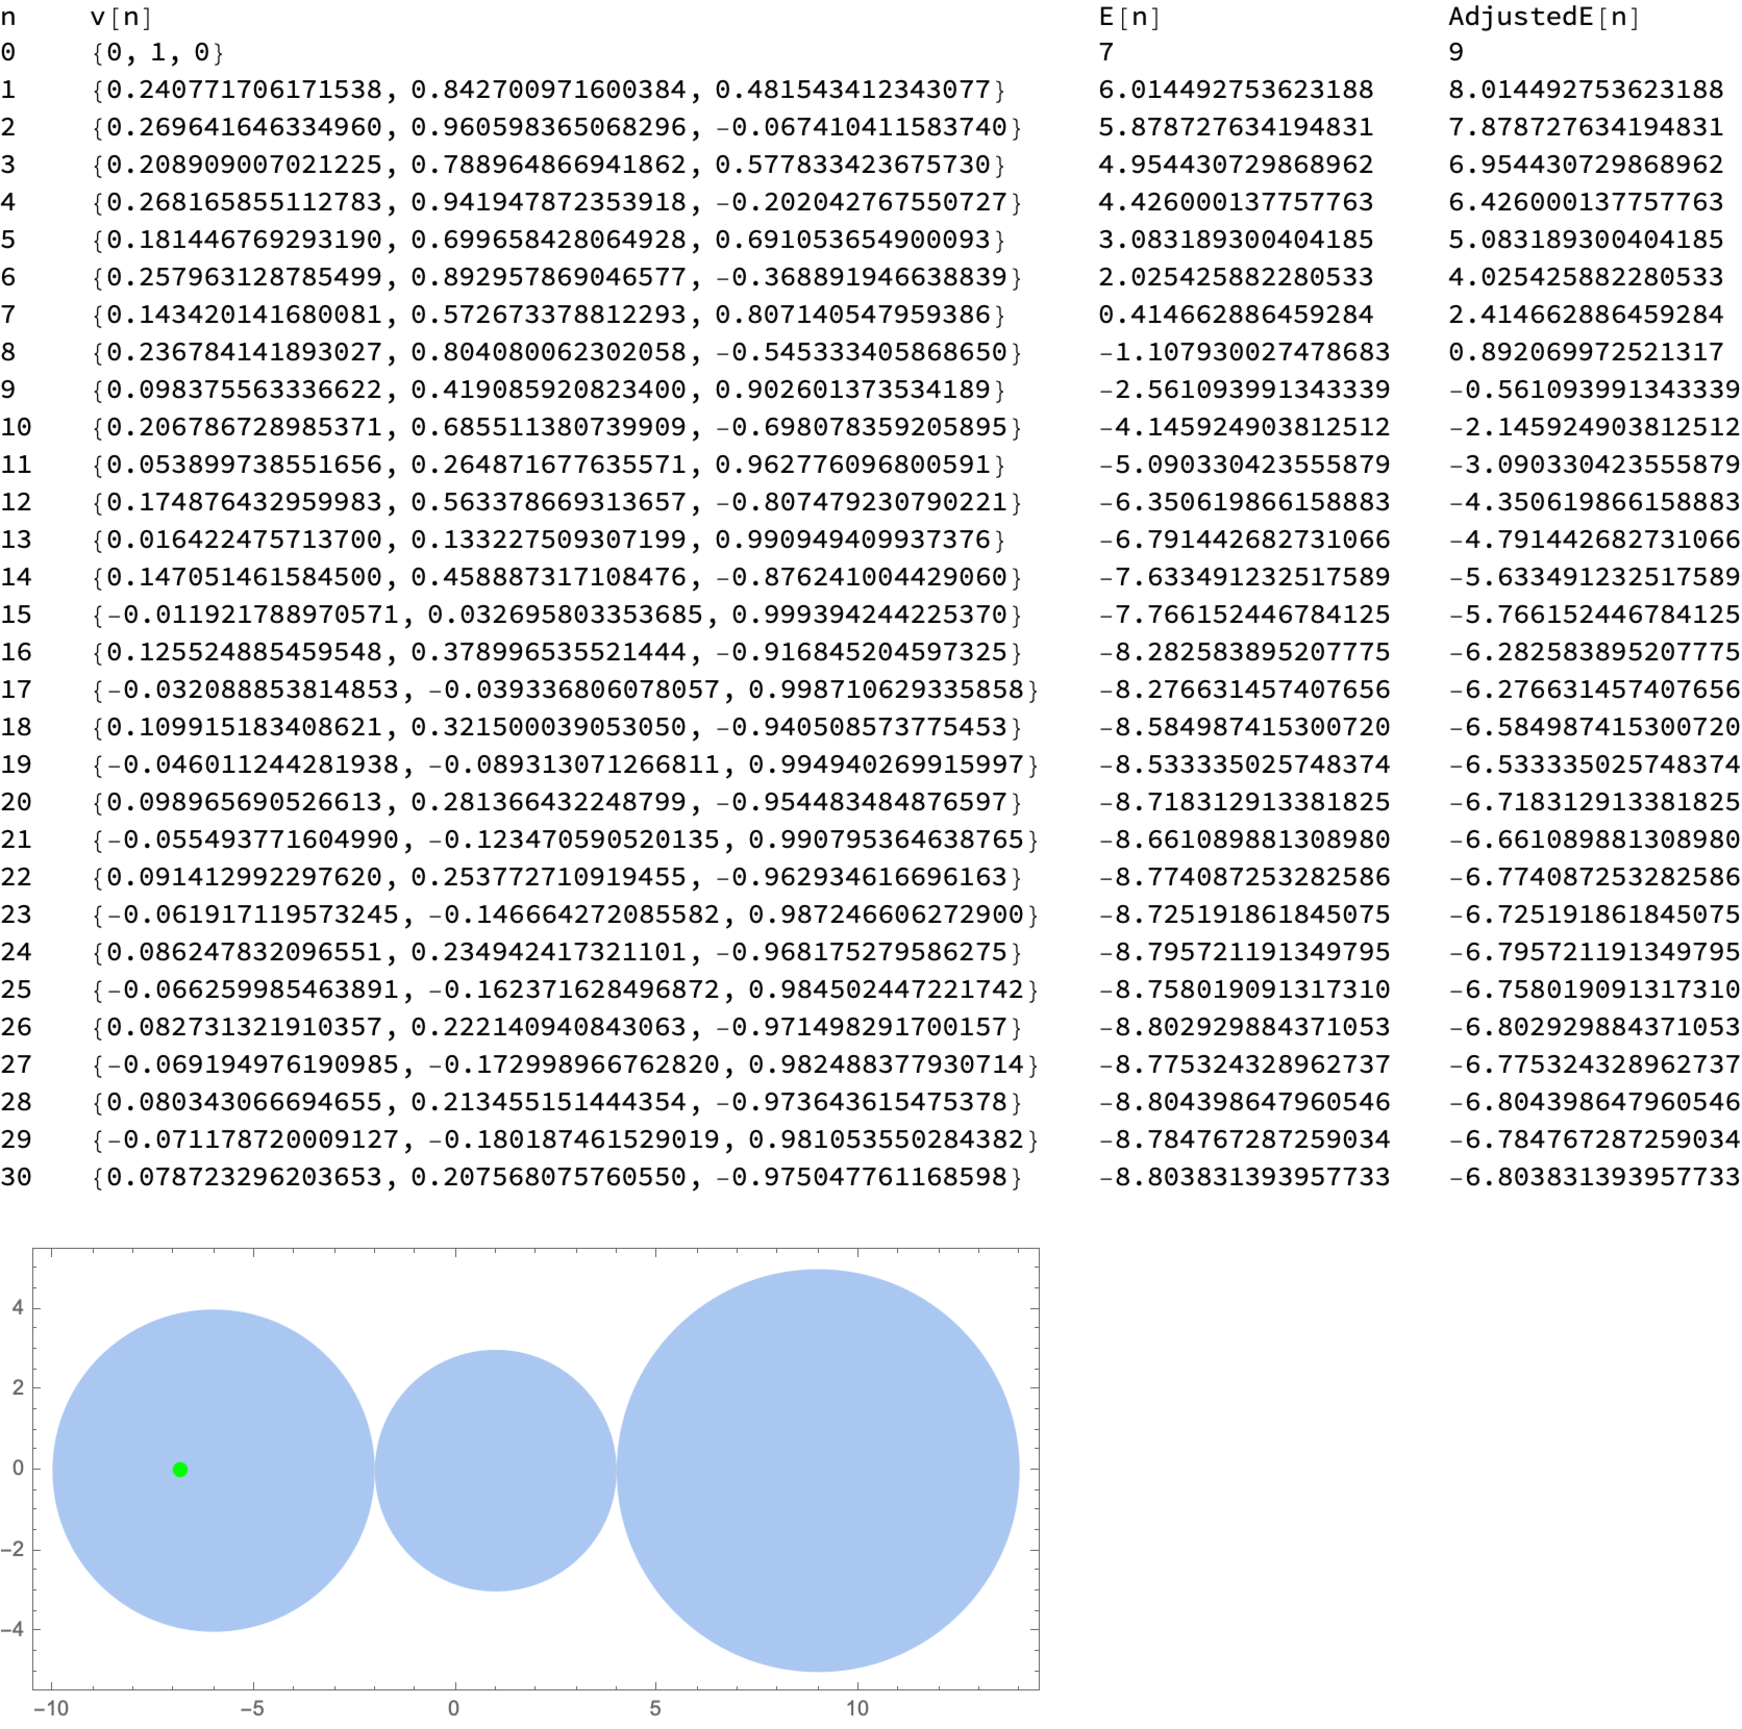
\includegraphics[scale=0.5]{problem52}

    \end{solution}
    
%%%%%%%%%%%%%%%%%%%%%%%%%%%%%%%%%%%%%%%%%%%%%%%%%%%%%%%%%%%%%
\end{document}